%!TEX root = ../thesis.tex
%*******************************************************************************
%****************************** Third Chapter **********************************
%*******************************************************************************
\chapter{Event reconstruction and selection}
During the proton collision, many types of processes happen whose information are saved in the CMS data storage system. But the events are only saved if they fulfill certain conditions compatible with the signal. 
For the tH process , the search is based on the presence of  a pair of muons with the same sign. The rest of the processes that also generates a pair of muons with the same sign will be considered backgrounds.  
\section{Signal Event Topology} 
In this search, top quark decays to $Wb$ and from the $W$ boson decays to a muon and a neutrino. The Higgs decays to a pair of opposite sign $W$ bosons, where one of the bosons can decay to a $\mu$ and its neutrino. This is the main process that generates events with two same sign muons.The tH process topology is shown in the figure \ref{jet}.\\

Figure \ref{jet}, also shows a b-jet that comes from the tH process.  Finally there is a forward  quark jet (highest $\eta$ value) generated from the initial collision. Additional jets or leptons can be generated from the other $W$ boson.
\\
	
  %The W bosons can also decay to quarks that generate jets. 
Due to the small cross section of the $tH$ process, the amount of $tH$ events is low compared to other Higgs production processes. 
Table \ref{tdecay} shows several processes that generate same sign muon events for $t$H. These numbers do not consider the detection efficiency.
  %But also tH process can generate the final states from $\tau$ decays but with a low probability. Some of them have probability near zero , but not impossible . %In graphics, these low probability processes would be very small figures that barely manifest.

%For the tH process, the largest contribution comes from Higgs decays to WW (about 75$\%$), followed
 %y $\tau \tau$ (about 20$\%$) and ZZ (about 5$\%$).

	\begin{figure}[!htbp]
		\centering
		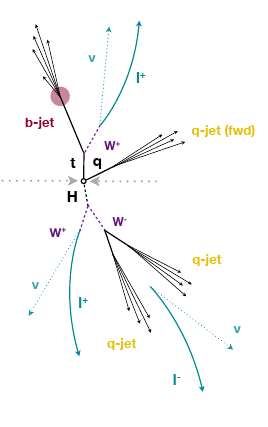
\includegraphics[scale=0.9]{Chapter1/jet.png}
		\caption{Topology of $t$H process which generates two same sign muons , a forward jet and a b-jet.} 
		\label{jet}
	\end{figure}
%Quarks and gluons only exist in bound states. Because of it, we cannot isolate quarks except the top quark because of their decay times that don't form a bound state. When two quarks are separated, the strong force interacting between them increases. The energy transforms into quark anti-quark pairs. The hadronization results in a jet of particles. 


\begin{table}[!ht]
	\caption{Expected number of events for different $tH$ decay chains assuming integrated luminosity of 35.9 fb$^{-1}$. $l$ represents $\mu^{\pm},e^\pm , \tau^\pm$.}
	\begin{tabular}{|l|c|c|}
		\hline
		Decay chain & BR & Events\\
		\hline 
		\small{$tH \rightarrow$ $W^+bW^+ W^-$ $\rightarrow$ $\mu^+$ $\nu_\mu b$ $\mu^+\nu_\mu$  $q \bar{q}'$ } &\small{2.096 $\times$10$^{-3}$} &  1.173  \\
		\hline
		\small{$tH \rightarrow W$$^+ b$$W^+$ $W^-$ $\rightarrow$ $\mu^+\nu_\mu b$ $\mu^+\nu_\mu$ $l^- \bar{\nu_l}$ } &\small{3.37 $\times$ 10$^{-4}$} &0.899 \\
		\hline
		\small{$tH \rightarrow$ $W^+ b$ $\tau^+ \tau^-$ $\rightarrow$ $\mu^+ \nu_\mu b$  $ \mu^+ \nu_\mu \bar{\nu_\tau} l^-\bar{\nu_l} \nu_\tau$} &\small{3.637$\times$10$^{-4}$}&0.203 \\
		\hline
		\small{$tH \rightarrow$ $W^+ b$ $W^+ W^-$ $\rightarrow$ $\tau^+ \bar{\nu_\tau}b$ $\mu^+ \nu_\mu$  $q\bar{q}$ $\rightarrow$ $\mu^+ \nu_\mu$ $\bar{\nu_\tau}$ $\bar{\nu_\tau} b\mu^+ \nu_\mu$  $q \bar{q}$} &\small{1.890$\times$10$^{-4}$}&0.105  \\
		\hline
		\small{$tH \rightarrow W^+ b \tau^+ \tau^-$ $\rightarrow$ $\mu^+$ $\nu_\mu b$ $\nu_\tau$ $\mu^+$ $\nu_\mu \bar{\nu_\tau}$} $q \bar{q}$  &
		\small{1.681 $\times$10$^{-4}$} & 0.094 \\
		\hline
		\small{$tH \rightarrow W^+ b$ $W^+ W^-$ $\rightarrow$ $\tau^+ \bar{\nu_\tau} b \mu^+ \nu_\mu l^- \bar{\nu_l}$ $\rightarrow$ $\mu^+\nu_\mu$ $ \bar{\nu_\tau} \bar{\nu_\tau} b \mu^+ \nu_\mu l^- \bar{\nu_l}$} &\small{3.045$\times$10$^{-5}$}& 0.017\\
		\hline
		\small{$tH \rightarrow W^+ bZZ$ $\rightarrow$ $q \bar{q} bZZ$ $\rightarrow$ $q \bar{q}  b \mu^+ \mu^- \mu^+ \mu^-$} & \small{1.966$\times$10$^{-5}$} &0.011\\
		\hline 
		\small{$tH \rightarrow$ $W^+ b$ $\tau^+ \tau^-$ $\rightarrow$ $\tau^+ \bar{\nu_\tau}b$ $\mu^+ \nu_\mu \bar{\nu_\tau} $  $q\bar{q}' \nu_\tau$ $\rightarrow$  $\mu^+ \nu_\mu \bar{\nu_\tau}\bar{\nu_\tau} b \mu^+ \nu_\mu \bar{\nu_\tau} $  $q\bar{q}' \nu_\tau$ } &\small{1.549 $\times$10$^{-5}$} &  0.008  \\
		\hline
	\end{tabular}
\label{tdecay}
\end{table}

\newpage


\section{Backgrounds}
Several processes contribute to the background in this search:
\begin{itemize}
		\item $\bm{t\bar{t}H}$: This Higgs  production mechanism is considered a background in this analysis. The muons in this cases comes from one top and Higgs decays. 
		\item $\bm{t\bar{t}W^{\pm}}$ and $\bm{t\bar{t}Z}$ $\bm{(t\bar{t}V)}$: One muons comes from a top and the other comes from the vector boson.
		\item $\bm{W^{\pm}W^{\pm}}$:A pair of same sign $W$ bosons generate a muon each one.
		\item $\bm{tZq}$: Processes with single top quarks associated  with a Z boson, where $Z\rightarrow \mu^+ \mu^-$, also contribute to the background.
	\item $\bm{t\bar{t}t\bar{t}}$:In these type of events, one $t$ decays to $Wb$ and $W$ decays to a muon. The second muon comes from the other top decay.
	%Backgrounds are estimated directly from simulated events$\%$ which are corrected for data/MC differences and $\%$ inefficiencies in the same way as signal events. 
		\item $\bm{ZZZ}$, $\bm{W^{+}ZZ}$ and $\bm{W^{+}W^{-}Z}$ ($\bm{VVV}$): The leptonic decays of the $W$ or $Z$ bosons generate at least two same sign muons.
	\item $\bm{WZ}$: Diboson production with leptonic decays. One muon comes from $W$ boson and the other from $Z$ boson.
	\item $\bm{tZW^{+}}$:One muon comes from the $Z$ while the other same sign muon can come from $t$ or $W$. 
	\item $\bm{ZZ}$: Each muon comes from $Z$ boson decays.
	\item $\bm{Fakes}$:This background refers to events where two muons come from  $b$ meson decays in jets.
\end{itemize}
Table \ref{back} show the decay chains and production cross section for background. 
\begin{table}
	\caption{Main backgrounds and their same sign $\mu\mu$ decay process }
	\centering
	\begin{tabular}{|c|l|}
		\hline
		Background &  Decay process \\
		\hline
		$t\bar{t}H$	& $t\bar{t}H$ $\rightarrow W^+b W^- \bar{b} W^+W^-$ $\rightarrow$ $\mu^+ \nu_\mu b$$\mu^- \bar{\nu_\mu}\bar{b}$ $\mu^+\nu_\mu$ $\mu^-\bar{\nu_\mu}$\\
		\hline  
		$t\bar{t}W$  &$t\bar{t}W$  $\rightarrow$  $W^+ b W^- \bar{b}$ $\mu^+\nu_\mu$ $\rightarrow$ $\mu^+ \nu_\mu b$ $\mu^- \bar{\nu_\mu} \bar{b}$ $\mu^+ \nu_\mu$\\
		\hline
		$t\bar{t} Z$ & $t\bar{t} Z$  $\rightarrow$ $W^+ b$  $W^-\bar{b} \mu^+ \mu^-$ $\rightarrow$ $\mu^+ \nu_\mu b$ $\mu^- \bar{\nu_\mu} \bar{b}\mu^+ \mu^-$  \\
		\hline 
		$W^\pm$ $W^\pm$  & $W^+W^+$ $\rightarrow$$\mu^+\nu_\mu$$\mu^+ {\nu_\mu}$ \\
		\hline 
		$tZq$  & $tZq$ $\rightarrow$ $W^+$ $ b\mu^+ \mu^- q$ $\rightarrow$$\mu^+ \nu_\mu b$ $\mu^+\mu^- q$ \\
		\hline 
		$t\bar{t}t\bar{t}$  &$t\bar{t}t\bar{t}$ $\rightarrow$ $W^+ b$   $W^- \bar{b}$  $W^+ b$  $W^- \bar{b}$   $\rightarrow$ $\mu^+ \nu_\mu b$ $\mu^- \bar{\nu_\mu} \bar{b}$ $\mu^+ \nu_\mu b$ $\mu^- \bar{\nu_\mu} \bar{b}$ \\
		\hline 
		$W^+ W^- Z$  &  $W^+ W^-$ $Z \rightarrow$ $\mu^+ \nu_\mu$ $\mu^- \bar{\nu_\mu} \mu^+ \mu^-$\\
		\hline 
		$ZZZ$  & $ZZZ \rightarrow$ $\mu^+ \mu^-\mu^+ \mu^-l^+ l^-$  \\
		\hline 
		$W^+ZZ$ &$W^+ZZ$ $\rightarrow$ $\mu^+ \nu_\mu \mu^+ \mu^- l^+l^-$ \\
		\hline 
		$W^+ Z$ &$W^+ Z \rightarrow$ $\mu^+ \nu_\mu \mu^+ \mu^-$ \\
		\hline
		$tZW^+$ & $tZW^+ \rightarrow$ $W^+b \mu^+ \mu^- \mu^+ \nu_\mu \rightarrow \mu^+ \nu_\mu b \mu^+ \mu^- \mu^+ \nu_\mu$\\
		\hline
		$ZZ$ &  $ZZ\rightarrow$ $\mu^+ \mu^- \mu^+ \mu^-$ \\
		\hline
	\end{tabular}
	\label{back}
\end{table} 
Due to small expected event yields, the processes $tZ$,$VVV$, $tzq$,$twz$ ,$W^\pm$ $W^\pm$ , $ZZ$ and $t\bar{t}t\bar{t}$ are grouped as one called Rares in the results below.
%Due to a large cross section, the main
%background contribution comes from WZ production.
\pagebreak

\section{Event Selection}
In order to detect signal events and reject background, the following selections are applied. 
\begin{itemize}
	\item The events must contain two muons with the same sign.
	\item Transverse moment $p_{t}$ > 25 GeV for the highest $p_t$ muon and $p_{t}$ > 15 GeV for the lowest $p_t$ muon.
	\item A forward jet with $p_t$ > 40 GeV and $|\eta|$ > 2.4
	\item One or more b tagged jets with  $|\eta|$ < 2.4
\end{itemize}
%Also it is possible to obtain a study of three leptons, given the mentioned decays can produce them. 
The number of events that passed the event selection are shown in figure \ref{tth-table} which corresponds to  a integrated luminosity of 35.9 fb$^{-1}$ \cite{th1}.\\

\begin{table}[ht!]
	\centering
\caption{Event yields for signal and backgrounds after the event selection for a integrated luminosity of 35.9 fb$^{-1}$}
	\begin{tabular}{|c|c|}
		\hline
		Process  & Number of events  \\
		\hline
			$tH$ & 2.14   \\
		\hline
		$t\bar{t}H$  &  24.18  \\
		\hline
		$t\bar{t}W$  &  68.03  \\
		\hline
		$t\bar{t}Z$  & 25.89 \\
		\hline
		Rares SM & 18.33  \\
		\hline
		$WZ$ & 15.07 \\
		\hline
		fakes  & 80.94 \\
		\hline
	\end{tabular}	
\label{tth-table}
\end{table}
The processes with the most events are $t\bar{t}$ $W^\pm$ and $t\bar{t}Z$. The number of events of Rares SM is the sum of the group of processes mentioned before. %$\kappa_t$ and $\kappa_V$ are coupling parameters. 
\pagebreak
%The fake rate corresponds to  non-prompt leptons.% Non prompt leptons are leptons that passed the selection, and usually comes from decays from b-jets (hadronized quarks). But due to jet signature is reconstructed as leptons, some particular signatures or errors in reconstruction, passed as leptons and then they called fakes leptons. Rare SM is a group of other processes: t$\bar{t}$t$\bar{t}$,WWW,WWZ,WZZ,WW,$t$Zq. Due to low number of events, they grouped the events as one histogram. 
\section{Boosted Decision Tree}
The Boosted Decision Tree (BDT) is a multivariate method that takes a set of input features and splits input data recursively based on
those features.  The features can be a mix of categorical and continuous data.
\\

Due to small signal to background ratio caused by the cross section of $t$H, a BDT  employed to train a discriminator to separate
tHq signal events from background . The BDT training is performed using several event variables for signal and background. In this case, the training was  based on $t\bar{t}V$, in order to discriminate $tH$, given  $t\bar{t}V$ has a higher number of events respect to $tH$ .\\
The variables used for the BDT were the following:

\begin{itemize}
	\item	$p_t$ of muon with lower momentum
	\item 	Total charge of tight leptons
	\item 	min $\Delta$R (lepton pairs)
	\item 	$\Delta\phi$ between highest $p_t$ lepton pair
	\item 	Number of jets with |$\eta$| < 2.4
	\item	Number of non b-tagged jets with |$\eta$| > 1.0
	\item	Maximum |$\eta$| for jets
	\item	$\Delta\eta$ (most forward light jet, closest lepton)
	\item	$\Delta\eta$ (most forward light jet, hardest loosely b-tagged jet)
	\item	$\Delta\eta$ (most forward light jet, 2nd hardest loosely b-tagged jet)
\end{itemize}


%Closure:  hay jets en los eventos de tt  (gluon-gluon -> tt + gluon ) que se pasan como muones.  jet -> muon =  fake

%Fakes:   proceso de QCD  que genera muchos  jets (por ejemplo  gluon-gluon -> gluons, quarks)  :    jet -> muons   fakes are estimated data 






